\documentclass{article}
\usepackage{graphicx}
\graphicspath{ {./images/} }

\title{Ch. 4 CW Pt. 1 Solns}
\author{Mr. Spence}
\date{\today}

\begin{document}

\maketitle

\begin{enumerate}

\item 

	\begin{enumerate}
	
	\item Having more children will increase people's taste for minivans and shift demand to the right. That increases the equilibrium price and quantity of minivans.
	\begin{figure}[h]
	\centering
	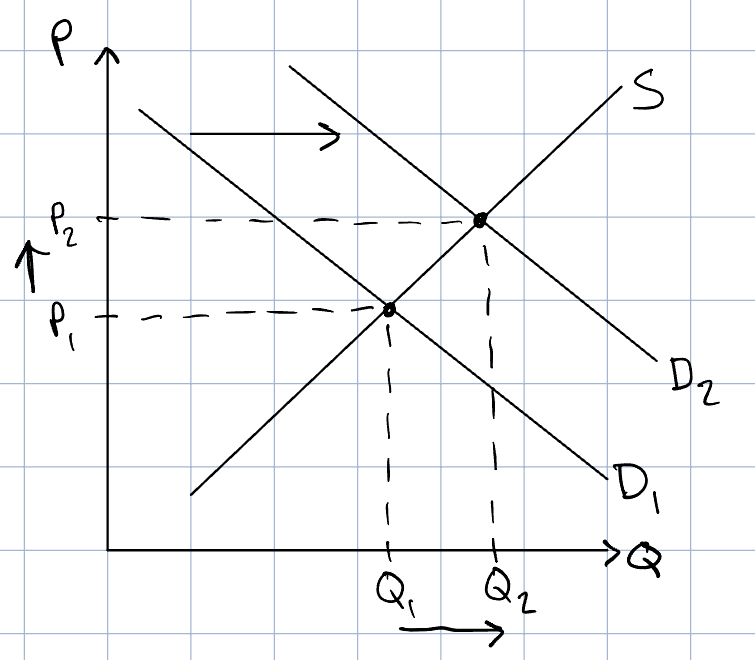
\includegraphics[width = 0.5\textwidth]{problem1a}
	\end{figure}
	
	\newpage	
	
	\item An input price has increased, so the supply of minivans will shift to the left. That increases equilibrium price and decreases equilibrium quantity.
	\begin{figure}[h]
	\centering
	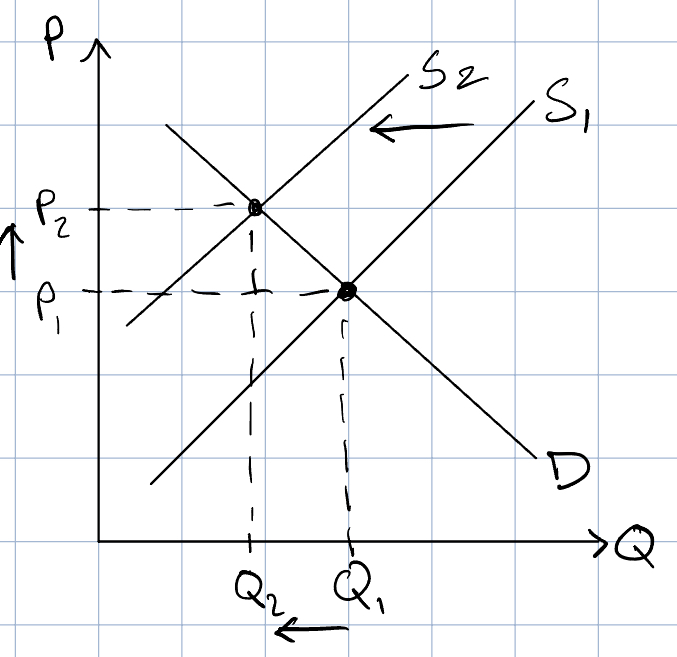
\includegraphics[width = 0.5\textwidth]{problem1b}
	\end{figure}
	
	\item The advancement in production technology will shift supply to the right which lowers the equilibrium price and raises the equilibrium quantity.
	\begin{figure}[h]
	\centering
	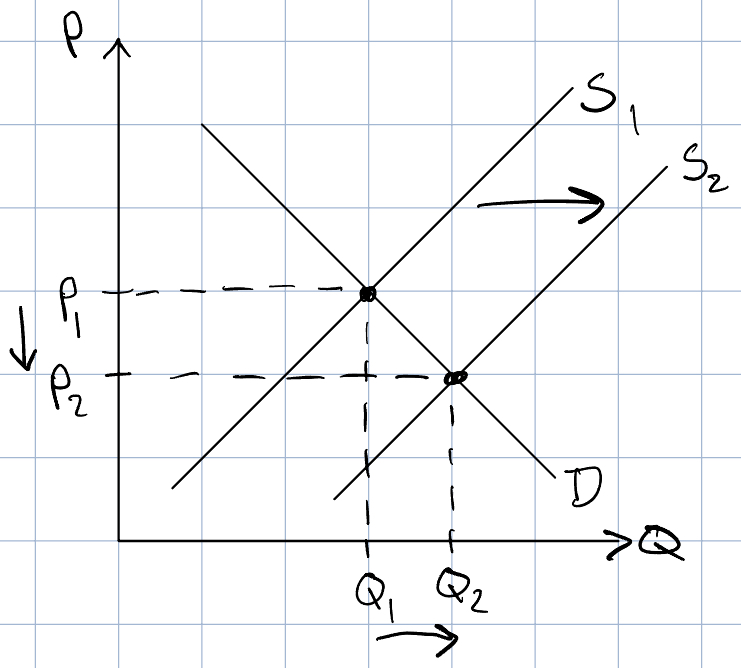
\includegraphics[width = 0.5\textwidth]{problem1c}
	\end{figure}
	
	\newpage
	
	\item SUVs are a substitute for minivans, so when they get more expensive, demand for minivans increases. That increases the equilibrium price and quantity of minivans.
	\begin{figure}[h]
	\centering
	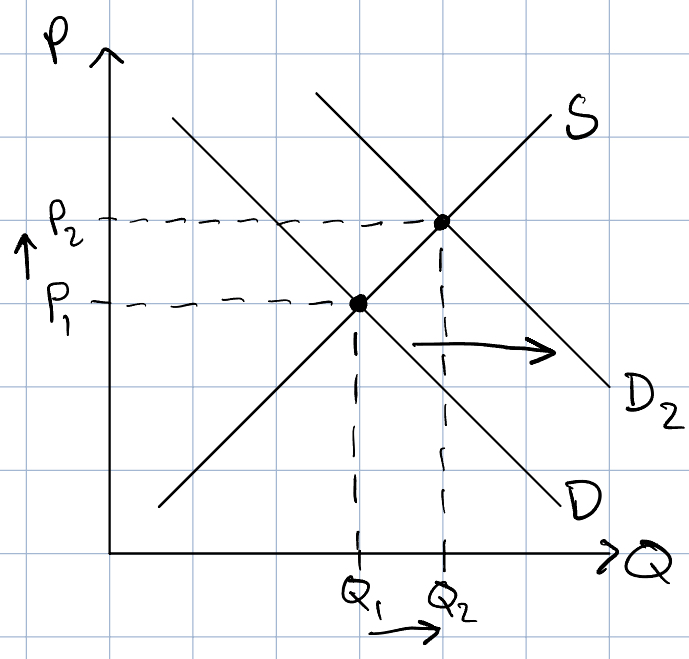
\includegraphics[width = 0.5\textwidth]{problem1d}
	\end{figure}
		
	\item Minivans are normal goods, so when incomes decline, people buy fewer minivans. That shifts demand to the left which lowers the equilibrium price and quantity. 
	\begin{figure}[h]
	\centering
	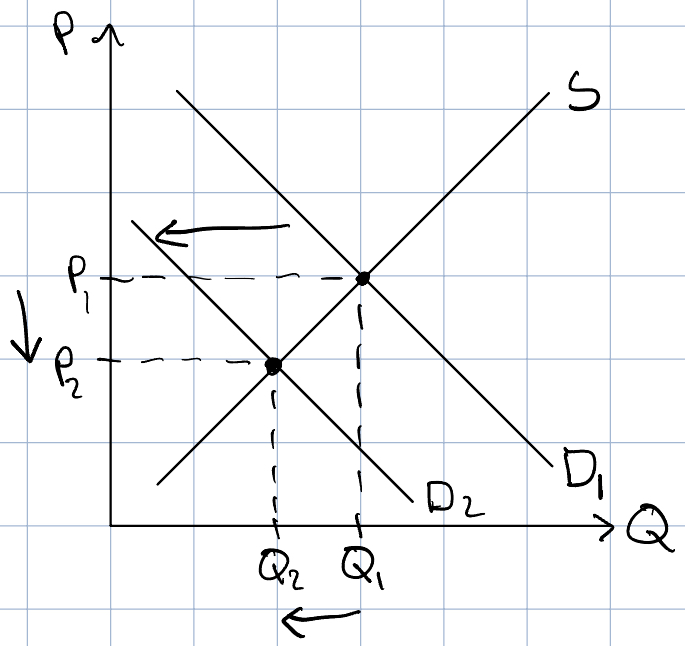
\includegraphics[width = 0.5\textwidth]{problem1e}
	\end{figure}
	
	\end{enumerate}
	
	\newpage

\item False -- After the increase in demand, the market will move towards equilibrium. That means quantity supplied will equal quantity demanded at a new, higher equilibrium quantity.

 	\begin{figure}[h]
	\centering
	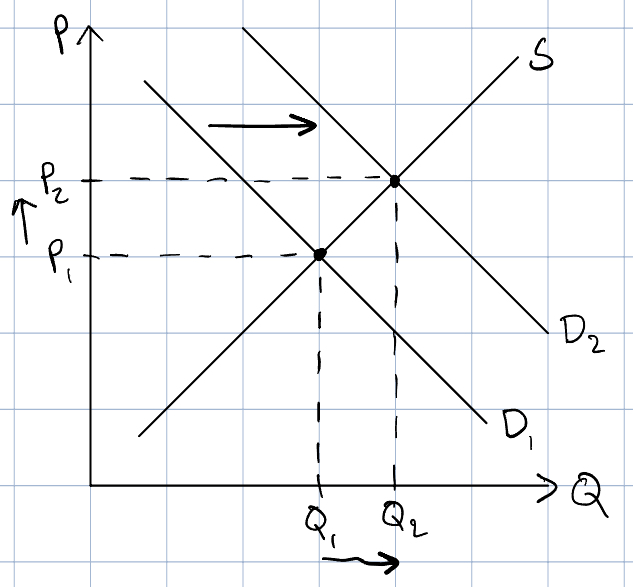
\includegraphics[width = 0.5\textwidth]{problem2}
	\end{figure}
	
\item

	\begin{enumerate}
	
	\item 
		
		\begin{itemize}
		
		\item Complements
		
		\item Substitutes
		
		\item Substitutes
		
		\end{itemize}
		
	\item The lower cost of manufacturing will shift the supply curve for TV screens to the right which decreases equilibrium price and increases equilibrium quantity.
	\begin{figure}[h]
	\centering
	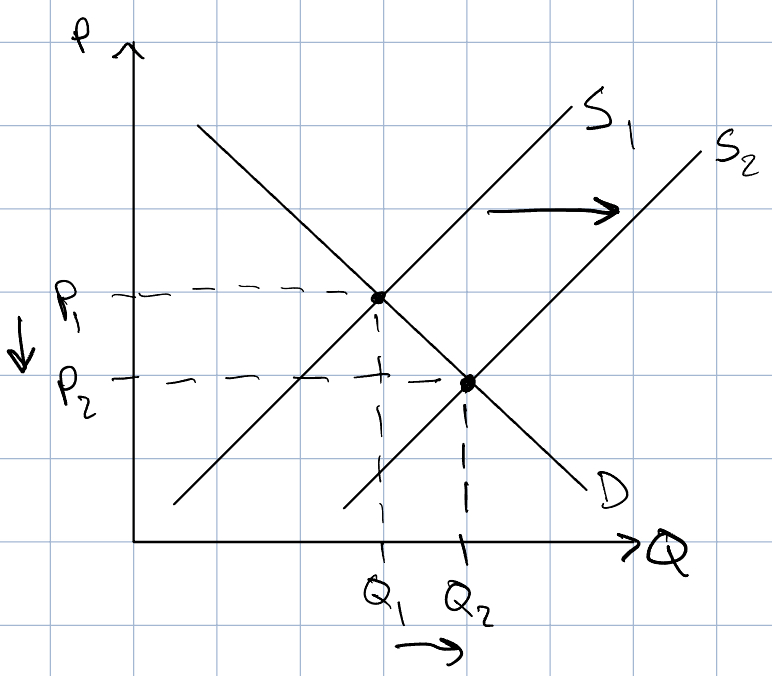
\includegraphics[width = 0.5\textwidth]{problem3b}
	\end{figure}
	
	\newpage
	
	\item Video streaming and TV screens are complements, so when the price of TV screens goes down, demand for streaming shifts right, price increases, and quantity increases.
	\begin{figure}[h]
	\centering
	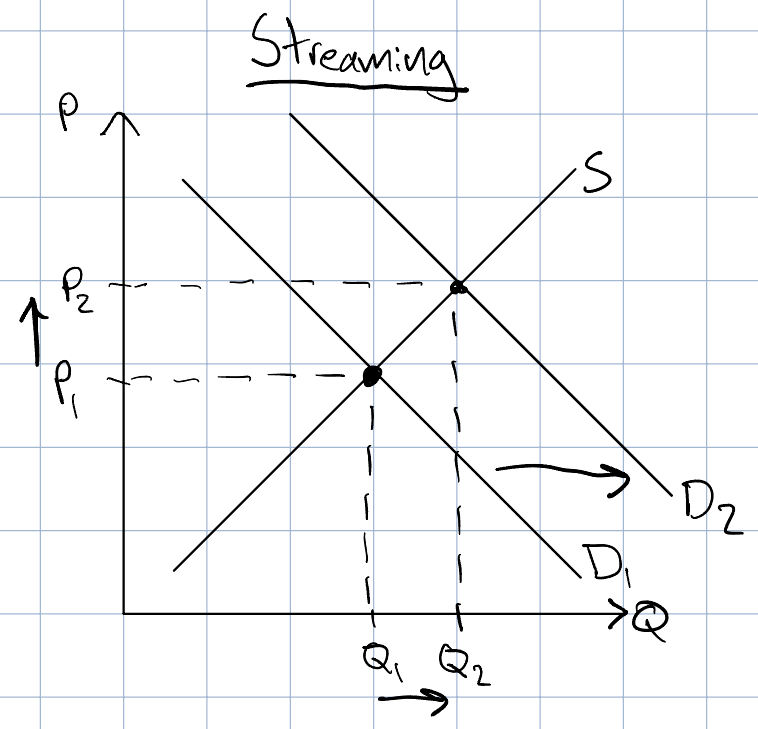
\includegraphics[width = 0.5\textwidth]{problem3c_streaming}
	\end{figure}
	
	Movie tickets and TV screens are substitutes, so when the price of TV screens goes down, demand for movie tickets shifts left, price decreases, and quantity decreases.
	\begin{figure}[h]
	\centering
	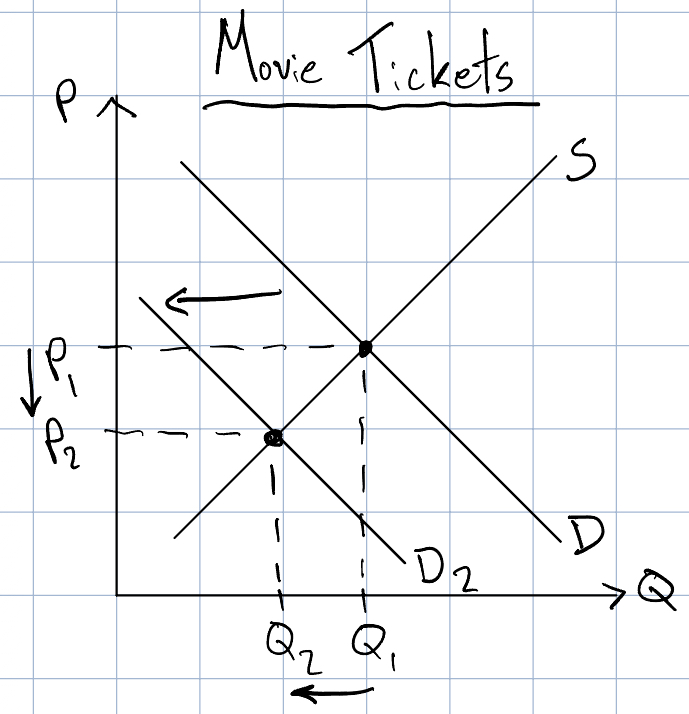
\includegraphics[width = 0.5\textwidth]{problem3c_tix}
	\end{figure}
	
	\end{enumerate}

\end{enumerate}

\end{document}
